\documentclass[twoside]{book}

% Packages required by doxygen
\usepackage{fixltx2e}
\usepackage{calc}
\usepackage{doxygen}
\usepackage[export]{adjustbox} % also loads graphicx
\usepackage{graphicx}
\usepackage[utf8]{inputenc}
\usepackage{makeidx}
\usepackage{multicol}
\usepackage{multirow}
\PassOptionsToPackage{warn}{textcomp}
\usepackage{textcomp}
\usepackage[nointegrals]{wasysym}
\usepackage[table]{xcolor}

% Font selection
\usepackage[T1]{fontenc}
\usepackage[scaled=.90]{helvet}
\usepackage{courier}
\usepackage{amssymb}
\usepackage{sectsty}
\renewcommand{\familydefault}{\sfdefault}
\allsectionsfont{%
  \fontseries{bc}\selectfont%
  \color{darkgray}%
}
\renewcommand{\DoxyLabelFont}{%
  \fontseries{bc}\selectfont%
  \color{darkgray}%
}
\newcommand{\+}{\discretionary{\mbox{\scriptsize$\hookleftarrow$}}{}{}}

% Page & text layout
\usepackage{geometry}
\geometry{%
  a4paper,%
  top=2.5cm,%
  bottom=2.5cm,%
  left=2.5cm,%
  right=2.5cm%
}
\tolerance=750
\hfuzz=15pt
\hbadness=750
\setlength{\emergencystretch}{15pt}
\setlength{\parindent}{0cm}
\setlength{\parskip}{0.2cm}
\makeatletter
\renewcommand{\paragraph}{%
  \@startsection{paragraph}{4}{0ex}{-1.0ex}{1.0ex}{%
    \normalfont\normalsize\bfseries\SS@parafont%
  }%
}
\renewcommand{\subparagraph}{%
  \@startsection{subparagraph}{5}{0ex}{-1.0ex}{1.0ex}{%
    \normalfont\normalsize\bfseries\SS@subparafont%
  }%
}
\makeatother

% Headers & footers
\usepackage{fancyhdr}
\pagestyle{fancyplain}
\fancyhead[LE]{\fancyplain{}{\bfseries\thepage}}
\fancyhead[CE]{\fancyplain{}{}}
\fancyhead[RE]{\fancyplain{}{\bfseries\leftmark}}
\fancyhead[LO]{\fancyplain{}{\bfseries\rightmark}}
\fancyhead[CO]{\fancyplain{}{}}
\fancyhead[RO]{\fancyplain{}{\bfseries\thepage}}
\fancyfoot[LE]{\fancyplain{}{}}
\fancyfoot[CE]{\fancyplain{}{}}
\fancyfoot[RE]{\fancyplain{}{\bfseries\scriptsize Generated on Wed Sep 30 2015 11\+:43\+:23 for My Project by Doxygen }}
\fancyfoot[LO]{\fancyplain{}{\bfseries\scriptsize Generated on Wed Sep 30 2015 11\+:43\+:23 for My Project by Doxygen }}
\fancyfoot[CO]{\fancyplain{}{}}
\fancyfoot[RO]{\fancyplain{}{}}
\renewcommand{\footrulewidth}{0.4pt}
\renewcommand{\chaptermark}[1]{%
  \markboth{#1}{}%
}
\renewcommand{\sectionmark}[1]{%
  \markright{\thesection\ #1}%
}

% Indices & bibliography
\usepackage{natbib}
\usepackage[titles]{tocloft}
\setcounter{tocdepth}{3}
\setcounter{secnumdepth}{5}
\makeindex

% Hyperlinks (required, but should be loaded last)
\usepackage{ifpdf}
\ifpdf
  \usepackage[pdftex,pagebackref=true]{hyperref}
\else
  \usepackage[ps2pdf,pagebackref=true]{hyperref}
\fi
\hypersetup{%
  colorlinks=true,%
  linkcolor=blue,%
  citecolor=blue,%
  unicode%
}

% Custom commands
\newcommand{\clearemptydoublepage}{%
  \newpage{\pagestyle{empty}\cleardoublepage}%
}


%===== C O N T E N T S =====

\begin{document}

% Titlepage & ToC
\hypersetup{pageanchor=false,
             bookmarks=true,
             bookmarksnumbered=true,
             pdfencoding=unicode
            }
\pagenumbering{roman}
\begin{titlepage}
\vspace*{7cm}
\begin{center}%
{\Large My Project }\\
\vspace*{1cm}
{\large Generated by Doxygen 1.8.10}\\
\vspace*{0.5cm}
{\small Wed Sep 30 2015 11:43:23}\\
\end{center}
\end{titlepage}
\clearemptydoublepage
\tableofcontents
\clearemptydoublepage
\pagenumbering{arabic}
\hypersetup{pageanchor=true}

%--- Begin generated contents ---
\chapter{Hierarchical Index}
\section{Class Hierarchy}
This inheritance list is sorted roughly, but not completely, alphabetically\+:\begin{DoxyCompactList}
\item \contentsline{section}{Cpsystem}{\pageref{class_cpsystem}}{}
\item \contentsline{section}{Key\+Signature}{\pageref{class_key_signature}}{}
\item \contentsline{section}{Note}{\pageref{class_note}}{}
\item Q\+Graphics\+Object\begin{DoxyCompactList}
\item \contentsline{section}{V\+Note}{\pageref{class_v_note}}{}
\item \contentsline{section}{V\+Staff}{\pageref{class_v_staff}}{}
\item \contentsline{section}{V\+Staff\+Line}{\pageref{class_v_staff_line}}{}
\end{DoxyCompactList}
\item Q\+Graphics\+View\begin{DoxyCompactList}
\item \contentsline{section}{Score\+View}{\pageref{class_score_view}}{}
\end{DoxyCompactList}
\item Q\+Main\+Window\begin{DoxyCompactList}
\item \contentsline{section}{Main\+Window}{\pageref{class_main_window}}{}
\end{DoxyCompactList}
\item \contentsline{section}{Score}{\pageref{class_score}}{}
\item \contentsline{section}{Score\+View\+Model}{\pageref{class_score_view_model}}{}
\item \contentsline{section}{Staff}{\pageref{class_staff}}{}
\item \contentsline{section}{Ui\+\_\+\+Main\+Window}{\pageref{class_ui___main_window}}{}
\begin{DoxyCompactList}
\item \contentsline{section}{Ui\+:\+:Main\+Window}{\pageref{class_ui_1_1_main_window}}{}
\end{DoxyCompactList}
\end{DoxyCompactList}

\chapter{Class Index}
\section{Class List}
Here are the classes, structs, unions and interfaces with brief descriptions\+:\begin{DoxyCompactList}
\item\contentsline{section}{\hyperlink{class_cpsystem}{Cpsystem} }{\pageref{class_cpsystem}}{}
\item\contentsline{section}{\hyperlink{class_key_signature}{Key\+Signature} }{\pageref{class_key_signature}}{}
\item\contentsline{section}{\hyperlink{class_ui_1_1_main_window}{Ui\+::\+Main\+Window} }{\pageref{class_ui_1_1_main_window}}{}
\item\contentsline{section}{\hyperlink{class_main_window}{Main\+Window} }{\pageref{class_main_window}}{}
\item\contentsline{section}{\hyperlink{class_new_staff_dialog}{New\+Staff\+Dialog} }{\pageref{class_new_staff_dialog}}{}
\item\contentsline{section}{\hyperlink{class_ui_1_1_new_staff_dialog}{Ui\+::\+New\+Staff\+Dialog} }{\pageref{class_ui_1_1_new_staff_dialog}}{}
\item\contentsline{section}{\hyperlink{class_note}{Note} }{\pageref{class_note}}{}
\item\contentsline{section}{\hyperlink{class_score}{Score} }{\pageref{class_score}}{}
\item\contentsline{section}{\hyperlink{class_score_view}{Score\+View} }{\pageref{class_score_view}}{}
\item\contentsline{section}{\hyperlink{class_score_view_model}{Score\+View\+Model} }{\pageref{class_score_view_model}}{}
\item\contentsline{section}{\hyperlink{class_staff}{Staff} }{\pageref{class_staff}}{}
\item\contentsline{section}{\hyperlink{class_ui___main_window}{Ui\+\_\+\+Main\+Window} }{\pageref{class_ui___main_window}}{}
\item\contentsline{section}{\hyperlink{class_ui___new_staff_dialog}{Ui\+\_\+\+New\+Staff\+Dialog} }{\pageref{class_ui___new_staff_dialog}}{}
\item\contentsline{section}{\hyperlink{class_v_note}{V\+Note} }{\pageref{class_v_note}}{}
\item\contentsline{section}{\hyperlink{class_v_staff}{V\+Staff} }{\pageref{class_v_staff}}{}
\item\contentsline{section}{\hyperlink{class_v_staff_line}{V\+Staff\+Line} }{\pageref{class_v_staff_line}}{}
\end{DoxyCompactList}

\chapter{Class Documentation}
\hypertarget{class_cpsystem}{}\section{Cpsystem Class Reference}
\label{class_cpsystem}\index{Cpsystem@{Cpsystem}}
\subsection*{Public Member Functions}
\begin{DoxyCompactItemize}
\item 
\hypertarget{class_cpsystem_ab113d039f9e7ff50e22983e7fc058c15}{}void {\bfseries test} ()\label{class_cpsystem_ab113d039f9e7ff50e22983e7fc058c15}

\item 
\hypertarget{class_cpsystem_ac5990c28fd6cf16617ef2a43f16ab194}{}\hyperlink{class_score_view_model}{Score\+View\+Model} $\ast$ {\bfseries get\+Scoreview} () const \label{class_cpsystem_ac5990c28fd6cf16617ef2a43f16ab194}

\item 
\hypertarget{class_cpsystem_ae0a0e675cc6dc034c601d92b9ca42ff8}{}int {\bfseries init\+Gui} (int argc, char $\ast$argv\mbox{[}$\,$\mbox{]})\label{class_cpsystem_ae0a0e675cc6dc034c601d92b9ca42ff8}

\end{DoxyCompactItemize}


The documentation for this class was generated from the following files\+:\begin{DoxyCompactItemize}
\item 
C\+:/\+Users/kollg/\+Documents/\+Git\+Hub/\+Counterpoint-\/project/cpsystem.\+h\item 
C\+:/\+Users/kollg/\+Documents/\+Git\+Hub/\+Counterpoint-\/project/cpsystem.\+cpp\end{DoxyCompactItemize}

\hypertarget{class_key_signature}{}\section{Key\+Signature Class Reference}
\label{class_key_signature}\index{Key\+Signature@{Key\+Signature}}
\subsection*{Public Member Functions}
\begin{DoxyCompactItemize}
\item 
\hypertarget{class_key_signature_ac3749df5c4d4bd6c11a1d9ce593da546}{}{\bfseries Key\+Signature} (int key=0)\label{class_key_signature_ac3749df5c4d4bd6c11a1d9ce593da546}

\item 
\hypertarget{class_key_signature_af773264a0f75f21635d35f037d0f5a46}{}int {\bfseries get\+Keysig} () const \label{class_key_signature_af773264a0f75f21635d35f037d0f5a46}

\item 
\hypertarget{class_key_signature_aa91751b71f480eec27f3e0215d11eada}{}void {\bfseries set\+Key\+Sig} (int key=0)\label{class_key_signature_aa91751b71f480eec27f3e0215d11eada}

\end{DoxyCompactItemize}


The documentation for this class was generated from the following files\+:\begin{DoxyCompactItemize}
\item 
C\+:/\+Users/kollg/\+Documents/\+Git\+Hub/\+Counterpoint-\/project/keysignature.\+h\item 
C\+:/\+Users/kollg/\+Documents/\+Git\+Hub/\+Counterpoint-\/project/keysignature.\+cpp\end{DoxyCompactItemize}

\hypertarget{class_ui_1_1_main_window}{}\section{Ui\+:\+:Main\+Window Class Reference}
\label{class_ui_1_1_main_window}\index{Ui\+::\+Main\+Window@{Ui\+::\+Main\+Window}}
Inheritance diagram for Ui\+:\+:Main\+Window\+:\begin{figure}[H]
\begin{center}
\leavevmode
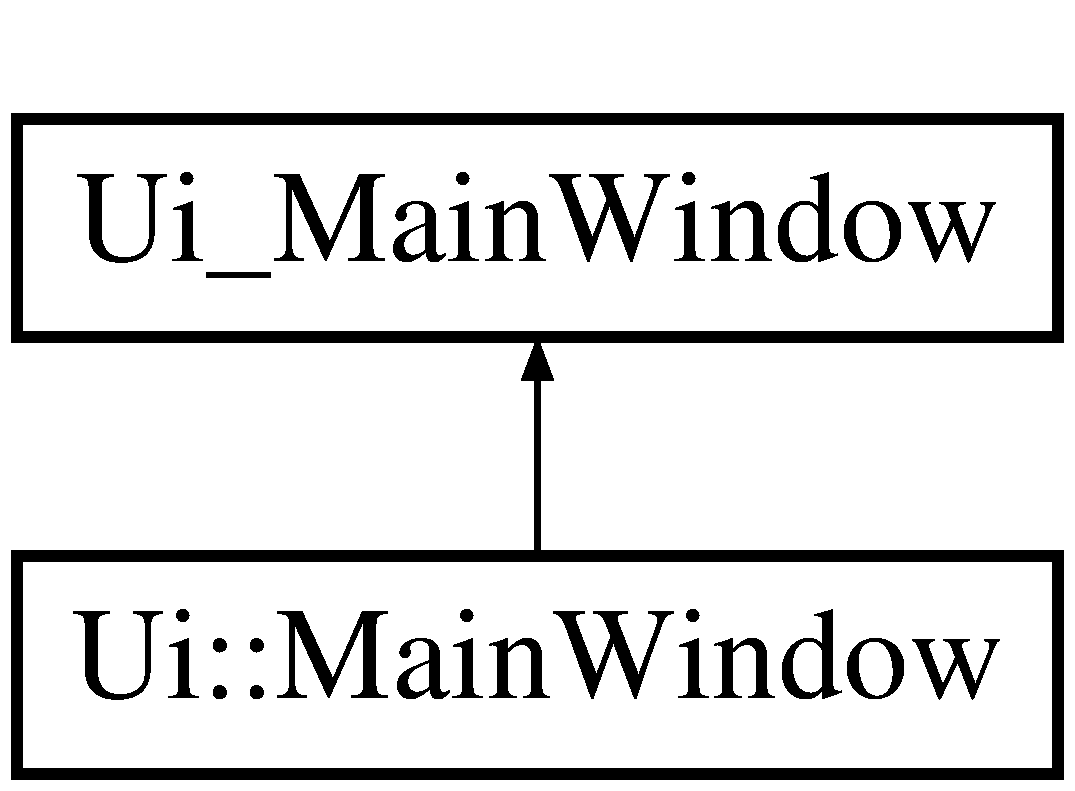
\includegraphics[height=2.000000cm]{class_ui_1_1_main_window}
\end{center}
\end{figure}
\subsection*{Additional Inherited Members}


The documentation for this class was generated from the following file\+:\begin{DoxyCompactItemize}
\item 
C\+:/\+Users/kollg/\+Documents/\+Git\+Hub/\+Counterpoint-\/project/ui\+\_\+mainwindow.\+h\end{DoxyCompactItemize}

\hypertarget{class_main_window}{}\section{Main\+Window Class Reference}
\label{class_main_window}\index{Main\+Window@{Main\+Window}}
Inheritance diagram for Main\+Window\+:\begin{figure}[H]
\begin{center}
\leavevmode
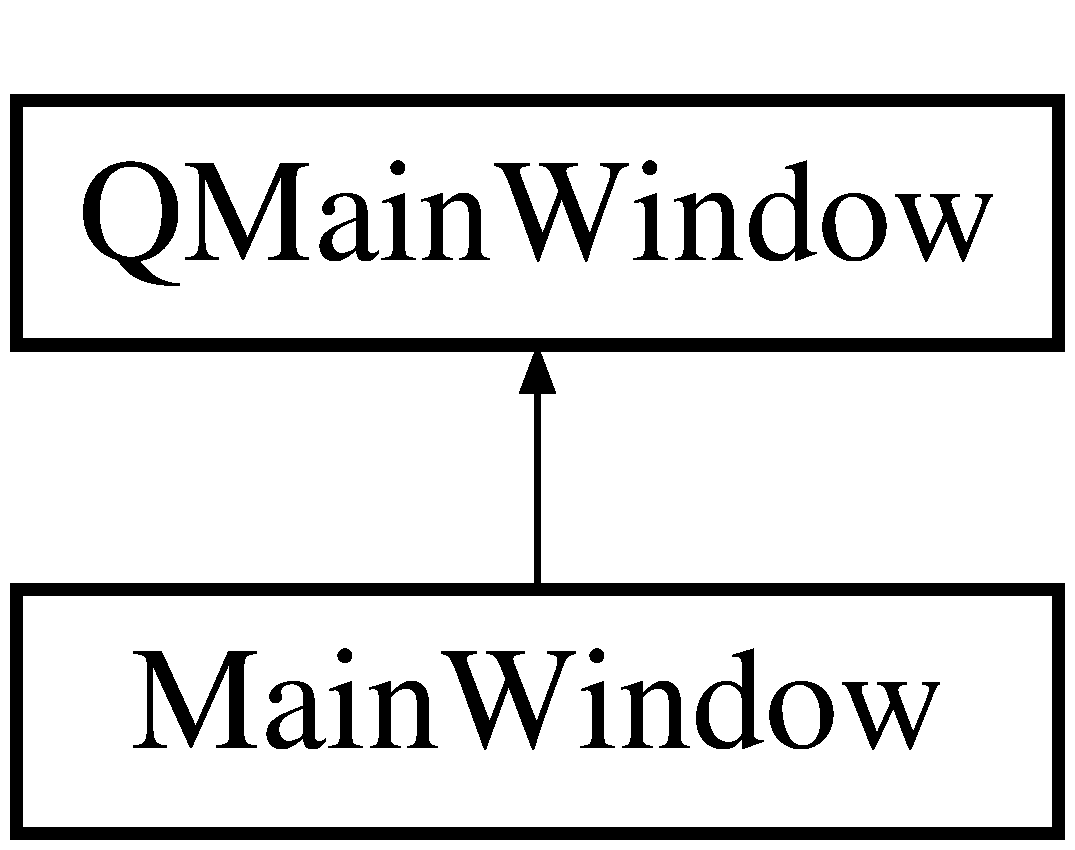
\includegraphics[height=2.000000cm]{class_main_window}
\end{center}
\end{figure}
\subsection*{Public Slots}
\begin{DoxyCompactItemize}
\item 
\hypertarget{class_main_window_a5efd5117f1bad9f03e909b6865099e5b}{}void {\bfseries v\+Note\+Selected} (\hyperlink{class_v_note}{V\+Note} $\ast$note)\label{class_main_window_a5efd5117f1bad9f03e909b6865099e5b}

\item 
\hypertarget{class_main_window_a2cf6671f3b110419e7d9704966334235}{}void {\bfseries v\+Note\+Pos\+Changed} (\hyperlink{class_v_note}{V\+Note} $\ast$note)\label{class_main_window_a2cf6671f3b110419e7d9704966334235}

\item 
\hypertarget{class_main_window_a6cd57f6ba7f45bc7f1e723aa99ada0f0}{}void {\bfseries vstaff\+Selected} (\hyperlink{class_v_staff}{V\+Staff} $\ast$vstaff)\label{class_main_window_a6cd57f6ba7f45bc7f1e723aa99ada0f0}

\item 
\hypertarget{class_main_window_ab76ad97e59b1bc8be3bf8dc05cc37ecb}{}void {\bfseries new\+V\+Note\+Added} (\hyperlink{class_v_note}{V\+Note} $\ast$vnote)\label{class_main_window_ab76ad97e59b1bc8be3bf8dc05cc37ecb}

\end{DoxyCompactItemize}
\subsection*{Public Member Functions}
\begin{DoxyCompactItemize}
\item 
\hypertarget{class_main_window_a8b244be8b7b7db1b08de2a2acb9409db}{}{\bfseries Main\+Window} (Q\+Widget $\ast$parent=0)\label{class_main_window_a8b244be8b7b7db1b08de2a2acb9409db}

\item 
\hypertarget{class_main_window_a24fce628de02495376e8c1724c077f2a}{}void {\bfseries set\+Svm} (\hyperlink{class_score_view_model}{Score\+View\+Model} $\ast$value)\label{class_main_window_a24fce628de02495376e8c1724c077f2a}

\item 
\hypertarget{class_main_window_a6634f1163a8752a689aa7ff6ffc0e4b1}{}void {\bfseries show\+Score} ()\label{class_main_window_a6634f1163a8752a689aa7ff6ffc0e4b1}

\item 
\hypertarget{class_main_window_a29b23178fefbc36a440072d0c9ded820}{}void {\bfseries show\+Next\+V\+Staff} (\hyperlink{class_v_staff}{V\+Staff} $\ast$vstaff)\label{class_main_window_a29b23178fefbc36a440072d0c9ded820}

\item 
\hypertarget{class_main_window_a4d8d7633f5fcbe11cd1a046301060b96}{}void {\bfseries update\+Note\+Data} (\hyperlink{class_v_note}{V\+Note} $\ast$vnote)\label{class_main_window_a4d8d7633f5fcbe11cd1a046301060b96}

\item 
\hypertarget{class_main_window_a11b07925a93ef53750a9da3993c05701}{}void {\bfseries add\+V\+Staff} (\hyperlink{class_v_staff}{V\+Staff} $\ast$vstaff)\label{class_main_window_a11b07925a93ef53750a9da3993c05701}

\item 
\hypertarget{class_main_window_a7345a180da85799035f01dda512ad8d3}{}Q\+List$<$ \hyperlink{class_v_staff}{V\+Staff} $\ast$ $>$ {\bfseries get\+Vstaffs} () const \label{class_main_window_a7345a180da85799035f01dda512ad8d3}

\end{DoxyCompactItemize}
\subsection*{Protected Member Functions}
\begin{DoxyCompactItemize}
\item 
\hypertarget{class_main_window_a9c4f542263838b9ecd06eae839a42a34}{}void {\bfseries key\+Press\+Event} (Q\+Key\+Event $\ast$event)\label{class_main_window_a9c4f542263838b9ecd06eae839a42a34}

\end{DoxyCompactItemize}


The documentation for this class was generated from the following files\+:\begin{DoxyCompactItemize}
\item 
C\+:/\+Users/kollg/\+Documents/\+Git\+Hub/\+Counterpoint-\/project/mainwindow.\+h\item 
C\+:/\+Users/kollg/\+Documents/\+Git\+Hub/\+Counterpoint-\/project/mainwindow.\+cpp\end{DoxyCompactItemize}

\hypertarget{class_new_staff_dialog}{}\section{New\+Staff\+Dialog Class Reference}
\label{class_new_staff_dialog}\index{New\+Staff\+Dialog@{New\+Staff\+Dialog}}
Inheritance diagram for New\+Staff\+Dialog\+:\begin{figure}[H]
\begin{center}
\leavevmode
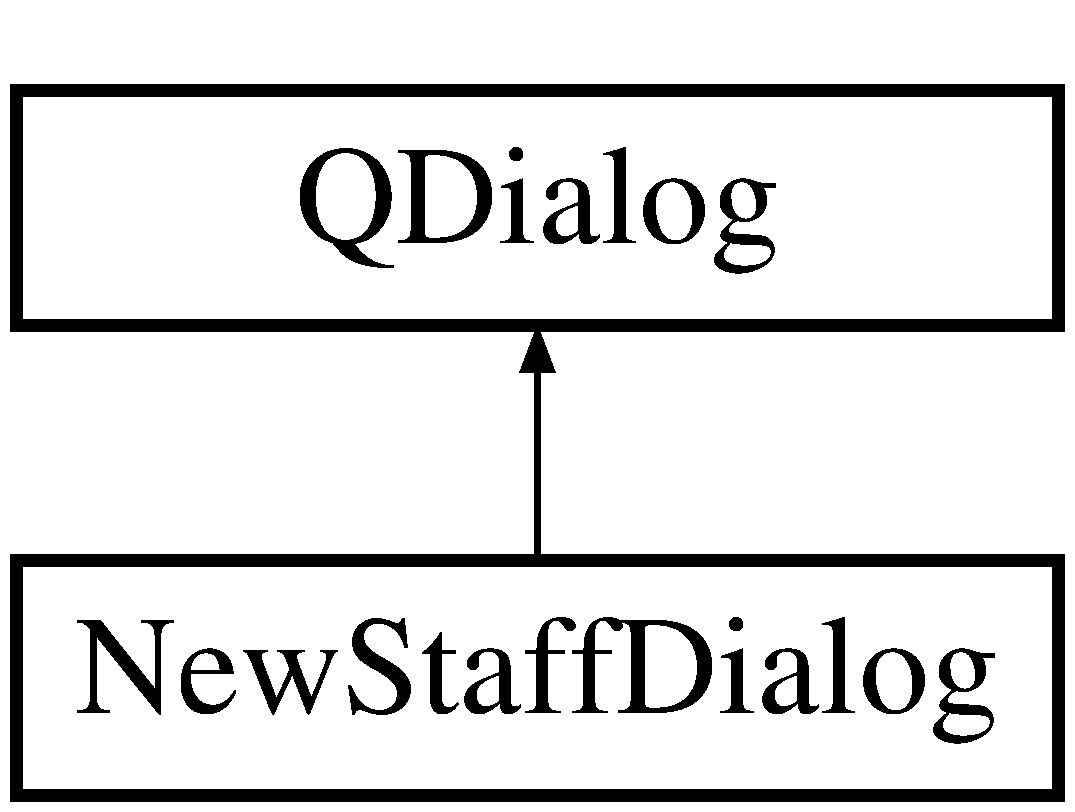
\includegraphics[height=2.000000cm]{class_new_staff_dialog}
\end{center}
\end{figure}
\subsection*{Public Member Functions}
\begin{DoxyCompactItemize}
\item 
\hypertarget{class_new_staff_dialog_a432b7b4d4dcf8cc9ef4ba91bd7a59eba}{}{\bfseries New\+Staff\+Dialog} (Q\+Widget $\ast$parent=0)\label{class_new_staff_dialog_a432b7b4d4dcf8cc9ef4ba91bd7a59eba}

\item 
\hypertarget{class_new_staff_dialog_a51da86da089ddc3b225c0ad3b2cdc64d}{}Score\+View\+Model\+::clef\+Names {\bfseries get\+Selectedclef} () const \label{class_new_staff_dialog_a51da86da089ddc3b225c0ad3b2cdc64d}

\item 
\hypertarget{class_new_staff_dialog_a0ecb9912f41ddaba3ade539bca33cd46}{}int {\bfseries get\+Selectedkeysignature} () const \label{class_new_staff_dialog_a0ecb9912f41ddaba3ade539bca33cd46}

\end{DoxyCompactItemize}


The documentation for this class was generated from the following files\+:\begin{DoxyCompactItemize}
\item 
C\+:/\+Users/kollg/\+Documents/\+Git\+Hub/\+Counterpoint-\/project/newstaffdialog.\+h\item 
C\+:/\+Users/kollg/\+Documents/\+Git\+Hub/\+Counterpoint-\/project/newstaffdialog.\+cpp\end{DoxyCompactItemize}

\hypertarget{class_ui_1_1_new_staff_dialog}{}\section{Ui\+:\+:New\+Staff\+Dialog Class Reference}
\label{class_ui_1_1_new_staff_dialog}\index{Ui\+::\+New\+Staff\+Dialog@{Ui\+::\+New\+Staff\+Dialog}}
Inheritance diagram for Ui\+:\+:New\+Staff\+Dialog\+:\begin{figure}[H]
\begin{center}
\leavevmode
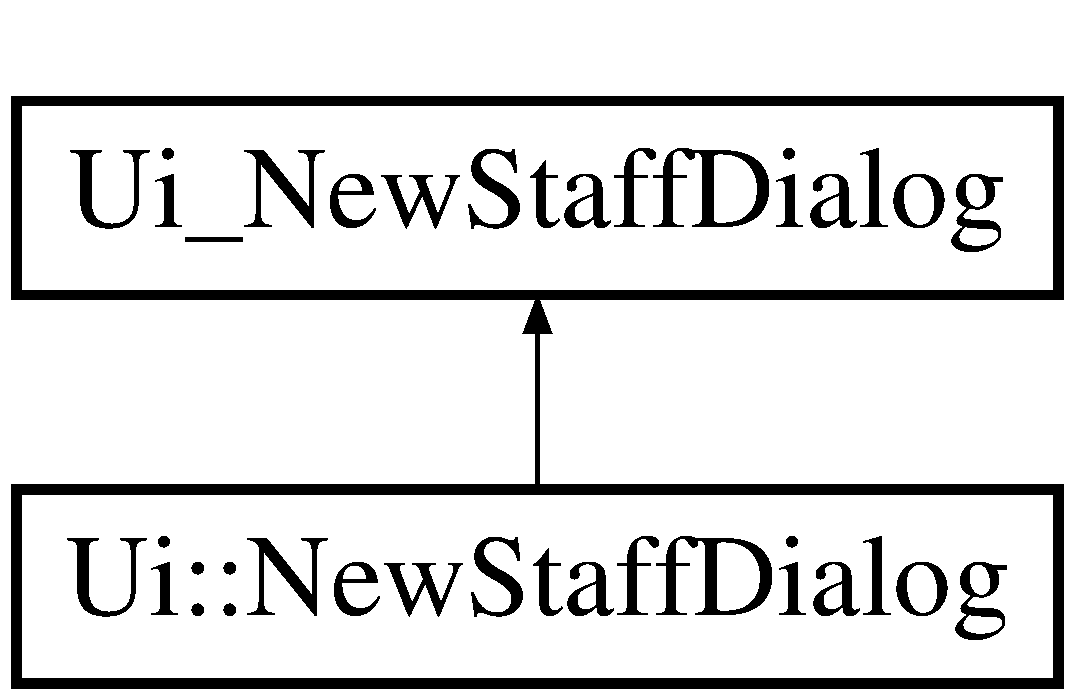
\includegraphics[height=2.000000cm]{class_ui_1_1_new_staff_dialog}
\end{center}
\end{figure}
\subsection*{Additional Inherited Members}


The documentation for this class was generated from the following file\+:\begin{DoxyCompactItemize}
\item 
C\+:/\+Users/kollg/\+Documents/\+Git\+Hub/\+Counterpoint-\/project/ui\+\_\+newstaffdialog.\+h\end{DoxyCompactItemize}

\hypertarget{class_note}{}\section{Note Class Reference}
\label{class_note}\index{Note@{Note}}
\subsection*{Public Member Functions}
\begin{DoxyCompactItemize}
\item 
\hypertarget{class_note_a15f24ce09b151698b706b10317dda8f5}{}{\bfseries Note} (int pi=Cpitch, int dur=4)\label{class_note_a15f24ce09b151698b706b10317dda8f5}

\item 
\hypertarget{class_note_a2bb5143ddd22a39471ecde82ad36ba1a}{}{\bfseries Note} (const \hyperlink{class_note}{Note} \&obj)\label{class_note_a2bb5143ddd22a39471ecde82ad36ba1a}

\item 
\hypertarget{class_note_adf42f07510d85bb1076f6e5dc6083d3c}{}int {\bfseries get\+Pitch} () const \label{class_note_adf42f07510d85bb1076f6e5dc6083d3c}

\item 
\hypertarget{class_note_ab542035784588db1d5be661414509af3}{}void {\bfseries set\+Pitch} (int value)\label{class_note_ab542035784588db1d5be661414509af3}

\item 
\hypertarget{class_note_aab9a1337e71fae0c910a2749516046f0}{}int {\bfseries get\+Duration} () const \label{class_note_aab9a1337e71fae0c910a2749516046f0}

\item 
\hypertarget{class_note_abb204bf93a2a3aea4237d6cf1638348f}{}void {\bfseries set\+Duration} (unsigned value)\label{class_note_abb204bf93a2a3aea4237d6cf1638348f}

\item 
\hypertarget{class_note_a5514ac8d4e41243402e4a6c59675059b}{}bool {\bfseries is\+Rest} () const \label{class_note_a5514ac8d4e41243402e4a6c59675059b}

\item 
\hypertarget{class_note_a59382ba872b863d7685fb6a864b66c24}{}void {\bfseries operator++} ()\label{class_note_a59382ba872b863d7685fb6a864b66c24}

\item 
\hypertarget{class_note_a1d1a0915b0957fa0461ccb35d8a355e8}{}void {\bfseries operator-\/-\/} ()\label{class_note_a1d1a0915b0957fa0461ccb35d8a355e8}

\item 
\hypertarget{class_note_a0f3c3cb7c09184974f9ffc43ae172e05}{}bool {\bfseries one\+Duration\+Up} ()\label{class_note_a0f3c3cb7c09184974f9ffc43ae172e05}

\item 
\hypertarget{class_note_a5ddfcb73da1e0690f7c1a9f0ceacd443}{}bool {\bfseries one\+Duration\+Down} ()\label{class_note_a5ddfcb73da1e0690f7c1a9f0ceacd443}

\item 
\hypertarget{class_note_a3f3527e444b1155ce16cbbaef24bcf91}{}int {\bfseries operator-\/} (const \hyperlink{class_note}{Note} \&other) const \label{class_note_a3f3527e444b1155ce16cbbaef24bcf91}

\item 
\hypertarget{class_note_a984fa9cde034c65bb365d2cd62b80652}{}bool {\bfseries operator==} (const \hyperlink{class_note}{Note} \&other) const \label{class_note_a984fa9cde034c65bb365d2cd62b80652}

\item 
\hypertarget{class_note_a095170ee6baa08ce011b914e630055b9}{}\hyperlink{class_note}{Note} \& {\bfseries operator=} (const \hyperlink{class_note}{Note} \&obj)\label{class_note_a095170ee6baa08ce011b914e630055b9}

\end{DoxyCompactItemize}
\subsection*{Static Public Attributes}
\begin{DoxyCompactItemize}
\item 
\hypertarget{class_note_ab43719e2af6ebfefb262d23b78f240ff}{}static int {\bfseries Cpitch} = 0\label{class_note_ab43719e2af6ebfefb262d23b78f240ff}

\item 
\hypertarget{class_note_a83b316633a96283960c3c58479a18a76}{}static int {\bfseries rest} = -\/32767\label{class_note_a83b316633a96283960c3c58479a18a76}

\end{DoxyCompactItemize}


The documentation for this class was generated from the following files\+:\begin{DoxyCompactItemize}
\item 
C\+:/\+Users/kollg/\+Documents/\+Git\+Hub/\+Counterpoint-\/project/note.\+h\item 
C\+:/\+Users/kollg/\+Documents/\+Git\+Hub/\+Counterpoint-\/project/note.\+cpp\end{DoxyCompactItemize}

\hypertarget{class_score}{}\section{Score Class Reference}
\label{class_score}\index{Score@{Score}}
\subsection*{Public Member Functions}
\begin{DoxyCompactItemize}
\item 
\hypertarget{class_score_ac56f72ee31f68529c690f722676b3845}{}{\bfseries Score} (const vector$<$ \hyperlink{class_staff}{Staff} $>$ \&staffs)\label{class_score_ac56f72ee31f68529c690f722676b3845}

\item 
\hypertarget{class_score_a43cf7511f3556f766fbfa44d083d6ff8}{}unsigned int {\bfseries get\+Num\+Of\+Staffs} () const \label{class_score_a43cf7511f3556f766fbfa44d083d6ff8}

\item 
\hypertarget{class_score_ab638c4f5b4d3ce33a170e9b4c0c378a6}{}unsigned int {\bfseries get\+Num\+Of\+Notes} (unsigned int staffnum)\label{class_score_ab638c4f5b4d3ce33a170e9b4c0c378a6}

\item 
\hypertarget{class_score_af345ed9d25768384695cbd8689d77955}{}void {\bfseries add\+Staff} (unsigned int where=0)\label{class_score_af345ed9d25768384695cbd8689d77955}

\item 
\hypertarget{class_score_a7db1897d68ccd5a51cb74374d0a8beb3}{}bool {\bfseries delete\+Staff} (unsigned int which)\label{class_score_a7db1897d68ccd5a51cb74374d0a8beb3}

\item 
\hypertarget{class_score_a9466b1c9802a429f9731ee1a332894b3}{}\hyperlink{class_staff}{Staff} \& {\bfseries get\+Staff\+By\+Num} (unsigned int which)\label{class_score_a9466b1c9802a429f9731ee1a332894b3}

\end{DoxyCompactItemize}


The documentation for this class was generated from the following files\+:\begin{DoxyCompactItemize}
\item 
C\+:/\+Users/kollg/\+Documents/\+Git\+Hub/\+Counterpoint-\/project/score.\+h\item 
C\+:/\+Users/kollg/\+Documents/\+Git\+Hub/\+Counterpoint-\/project/score.\+cpp\end{DoxyCompactItemize}

\hypertarget{class_score_view}{}\section{Score\+View Class Reference}
\label{class_score_view}\index{Score\+View@{Score\+View}}
Inheritance diagram for Score\+View\+:\begin{figure}[H]
\begin{center}
\leavevmode
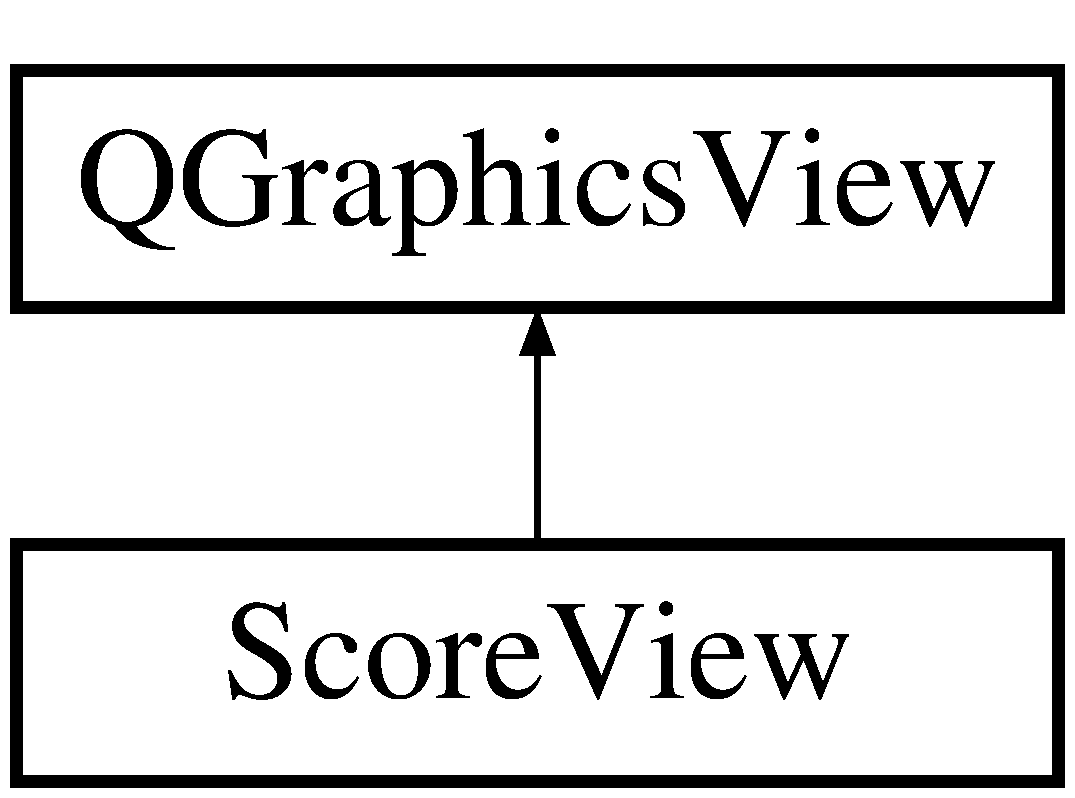
\includegraphics[height=2.000000cm]{class_score_view}
\end{center}
\end{figure}
\subsection*{Public Member Functions}
\begin{DoxyCompactItemize}
\item 
\hypertarget{class_score_view_a4bdafcdab114a507f0cef34ae23d23f3}{}{\bfseries Score\+View} (Q\+Widget $\ast$parent=0)\label{class_score_view_a4bdafcdab114a507f0cef34ae23d23f3}

\end{DoxyCompactItemize}
\subsection*{Protected Member Functions}
\begin{DoxyCompactItemize}
\item 
\hypertarget{class_score_view_a86954c336f05821fa615ba0f037dd16a}{}virtual void {\bfseries wheel\+Event} (Q\+Wheel\+Event $\ast$event)\label{class_score_view_a86954c336f05821fa615ba0f037dd16a}

\end{DoxyCompactItemize}


The documentation for this class was generated from the following files\+:\begin{DoxyCompactItemize}
\item 
C\+:/\+Users/kollg/\+Documents/\+Git\+Hub/\+Counterpoint-\/project/scoreview.\+h\item 
C\+:/\+Users/kollg/\+Documents/\+Git\+Hub/\+Counterpoint-\/project/scoreview.\+cpp\end{DoxyCompactItemize}

\hypertarget{class_score_view_model}{}\section{Score\+View\+Model Class Reference}
\label{class_score_view_model}\index{Score\+View\+Model@{Score\+View\+Model}}
\subsection*{Public Types}
\begin{DoxyCompactItemize}
\item 
\hypertarget{class_score_view_model_a2e603d26e71fb126b64895ae0b1636d2}{}enum {\bfseries clef\+Names} \{ {\bfseries treble}, 
{\bfseries alto}, 
{\bfseries tenor}, 
{\bfseries bass}
 \}\label{class_score_view_model_a2e603d26e71fb126b64895ae0b1636d2}

\item 
\hypertarget{class_score_view_model_a8b24e5bf70ec80a749d798cb7e907964}{}enum {\bfseries accents} \{ {\bfseries flat}, 
{\bfseries none}, 
{\bfseries sharp}, 
{\bfseries natural}
 \}\label{class_score_view_model_a8b24e5bf70ec80a749d798cb7e907964}

\item 
\hypertarget{class_score_view_model_a8e5435988383d8b15ff30eb41f1c0a5d}{}enum {\bfseries note\+Types} \{ \\*
{\bfseries whole\+\_\+rest}, 
{\bfseries half\+\_\+rest}, 
{\bfseries quarter\+\_\+rest}, 
{\bfseries eight\+\_\+rest}, 
\\*
{\bfseries whole}, 
{\bfseries half}, 
{\bfseries quarter}, 
{\bfseries eight}
 \}\label{class_score_view_model_a8e5435988383d8b15ff30eb41f1c0a5d}

\end{DoxyCompactItemize}
\subsection*{Public Member Functions}
\begin{DoxyCompactItemize}
\item 
\hypertarget{class_score_view_model_a2e95a5f0786d42535d04eeaa173ef90f}{}unsigned int {\bfseries get\+Num\+Of\+Staffs} () const \label{class_score_view_model_a2e95a5f0786d42535d04eeaa173ef90f}

\item 
\hypertarget{class_score_view_model_aba57d53f1f981ed6426362e72f314112}{}void {\bfseries add\+Staff} (clef\+Names clef=treble, int keysig=0, unsigned int where=0)\label{class_score_view_model_aba57d53f1f981ed6426362e72f314112}

\item 
\hypertarget{class_score_view_model_a48ec38e418000ba3e1f69678eaedaeee}{}void {\bfseries delete\+Staff} (unsigned int which)\label{class_score_view_model_a48ec38e418000ba3e1f69678eaedaeee}

\item 
\hypertarget{class_score_view_model_a89a469259de6149a1eb88faaae00b0b2}{}clef\+Names {\bfseries get\+Clef\+By\+Num} (int which)\label{class_score_view_model_a89a469259de6149a1eb88faaae00b0b2}

\item 
\hypertarget{class_score_view_model_a72a684c084554c68762d70e5a7bbf09c}{}void {\bfseries add\+Note} (unsigned int staffnum, int pitch, int duration, accents accent, unsigned int where=0)\label{class_score_view_model_a72a684c084554c68762d70e5a7bbf09c}

\item 
\hypertarget{class_score_view_model_a68c1b40e40541dbfc0ffd2194ca5bcb4}{}bool {\bfseries delete\+Note} (unsigned int staffnum, unsigned int which)\label{class_score_view_model_a68c1b40e40541dbfc0ffd2194ca5bcb4}

\item 
\hypertarget{class_score_view_model_a36c92215c16d908f3fd69093e4d307aa}{}\hyperlink{class_note}{Note} \& {\bfseries get\+Note\+By\+Num} (unsigned int staffnum, unsigned int which)\label{class_score_view_model_a36c92215c16d908f3fd69093e4d307aa}

\item 
\hypertarget{class_score_view_model_afd65004f27e1f03a7aab8c1c9b6635e4}{}unsigned int {\bfseries get\+Num\+Of\+Notes} (unsigned int staffnum) const \label{class_score_view_model_afd65004f27e1f03a7aab8c1c9b6635e4}

\item 
\hypertarget{class_score_view_model_adc09e48006e07d05cd06d28f85731ec4}{}void {\bfseries transpose} (int interval)\label{class_score_view_model_adc09e48006e07d05cd06d28f85731ec4}

\item 
\hypertarget{class_score_view_model_afc656d3b87cfcab65e2e2df84275811d}{}int {\bfseries get\+Position} (unsigned int staffnumber, unsigned int notenumber)\label{class_score_view_model_afc656d3b87cfcab65e2e2df84275811d}

\item 
\hypertarget{class_score_view_model_ac9ba2d57c16d6e20f4c3da111b73615f}{}accents {\bfseries get\+Accent} (unsigned int staffnumber, unsigned int notenumber)\label{class_score_view_model_ac9ba2d57c16d6e20f4c3da111b73615f}

\item 
\hypertarget{class_score_view_model_a6714358745b284c08d6cec01449ff306}{}note\+Types {\bfseries get\+Type} (unsigned int staffnumber, unsigned int notenumber)\label{class_score_view_model_a6714358745b284c08d6cec01449ff306}

\item 
\hypertarget{class_score_view_model_ab83b04a6d5678338e8b5712d5715048d}{}void {\bfseries update\+Position} (unsigned int staffnumber, unsigned int notenumber, int newscorepos)\label{class_score_view_model_ab83b04a6d5678338e8b5712d5715048d}

\item 
\hypertarget{class_score_view_model_a634fd237d616540d5031a64a72d3ddbf}{}void {\bfseries update\+Accent} (unsigned int staffnumber, unsigned int notenumber, accents newaccent)\label{class_score_view_model_a634fd237d616540d5031a64a72d3ddbf}

\item 
\hypertarget{class_score_view_model_ad78152fc30e09d58422e4671462d5884}{}void {\bfseries update\+Type} (unsigned int staffnumber, unsigned int notenumber, note\+Types newnotetype)\label{class_score_view_model_ad78152fc30e09d58422e4671462d5884}

\item 
\hypertarget{class_score_view_model_ac2247ce41cb07e55d007819e55dbc47b}{}void {\bfseries change\+To\+Rest} (unsigned int staffnumber, unsigned int notenumber)\label{class_score_view_model_ac2247ce41cb07e55d007819e55dbc47b}

\item 
\hypertarget{class_score_view_model_a99a64a7bd6e22a14eaf2920c44b1ca4a}{}void {\bfseries make\+Lily\+Pond} (Q\+String destination)\label{class_score_view_model_a99a64a7bd6e22a14eaf2920c44b1ca4a}

\item 
\hypertarget{class_score_view_model_a2ddc643ffec7b39df6e6b5fab7ab9e66}{}void {\bfseries read\+Lily\+Pond} (Q\+String file)\label{class_score_view_model_a2ddc643ffec7b39df6e6b5fab7ab9e66}

\end{DoxyCompactItemize}


The documentation for this class was generated from the following files\+:\begin{DoxyCompactItemize}
\item 
C\+:/\+Users/kollg/\+Documents/\+Git\+Hub/\+Counterpoint-\/project/scoreviewmodel.\+h\item 
C\+:/\+Users/kollg/\+Documents/\+Git\+Hub/\+Counterpoint-\/project/scoreviewmodel.\+cpp\end{DoxyCompactItemize}

\hypertarget{class_staff}{}\section{Staff Class Reference}
\label{class_staff}\index{Staff@{Staff}}
\subsection*{Public Member Functions}
\begin{DoxyCompactItemize}
\item 
\hypertarget{class_staff_a0d21fcb11e76001f4ecd84e29deff46f}{}{\bfseries Staff} (const vector$<$ \hyperlink{class_note}{Note} $>$ \&notes)\label{class_staff_a0d21fcb11e76001f4ecd84e29deff46f}

\item 
\hypertarget{class_staff_ac0fee1d59feb2dbed7948288f33e5638}{}{\bfseries Staff} (const \hyperlink{class_staff}{Staff} \&obj)\label{class_staff_ac0fee1d59feb2dbed7948288f33e5638}

\item 
\hypertarget{class_staff_ad310fdd73d8b93019886dfb9bae1d0f3}{}void {\bfseries add\+Note} (int pitch, int duration, unsigned int where=0)\label{class_staff_ad310fdd73d8b93019886dfb9bae1d0f3}

\item 
\hypertarget{class_staff_a84311488f013f1ea290e4fbb0e18fa72}{}bool {\bfseries delete\+Note} (unsigned int which)\label{class_staff_a84311488f013f1ea290e4fbb0e18fa72}

\item 
\hypertarget{class_staff_aff07431f7ea2dd8e5c67dd2d96ab9a71}{}\hyperlink{class_note}{Note} \& {\bfseries get\+Note\+By\+Num} (unsigned int which)\label{class_staff_aff07431f7ea2dd8e5c67dd2d96ab9a71}

\item 
\hypertarget{class_staff_ab404828c4ae9da75c5ca37d3eeaa980c}{}unsigned int {\bfseries get\+Num\+Of\+Notes} () const \label{class_staff_ab404828c4ae9da75c5ca37d3eeaa980c}

\item 
\hypertarget{class_staff_acda41e19d6385d0b7c721dc1cc437f66}{}void {\bfseries transpose} (int interval)\label{class_staff_acda41e19d6385d0b7c721dc1cc437f66}

\end{DoxyCompactItemize}


The documentation for this class was generated from the following files\+:\begin{DoxyCompactItemize}
\item 
C\+:/\+Users/kollg/\+Documents/\+Git\+Hub/\+Counterpoint-\/project/staff.\+h\item 
C\+:/\+Users/kollg/\+Documents/\+Git\+Hub/\+Counterpoint-\/project/staff.\+cpp\end{DoxyCompactItemize}

\hypertarget{class_ui___main_window}{}\section{Ui\+\_\+\+Main\+Window Class Reference}
\label{class_ui___main_window}\index{Ui\+\_\+\+Main\+Window@{Ui\+\_\+\+Main\+Window}}
Inheritance diagram for Ui\+\_\+\+Main\+Window\+:\begin{figure}[H]
\begin{center}
\leavevmode
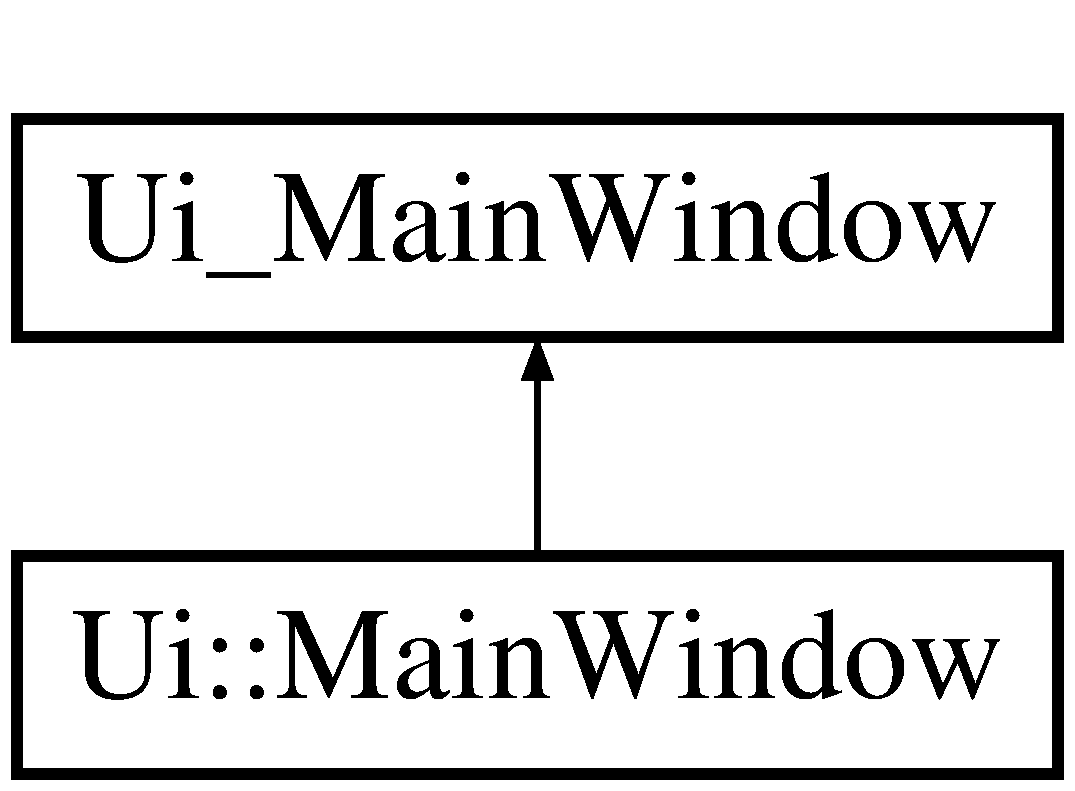
\includegraphics[height=2.000000cm]{class_ui___main_window}
\end{center}
\end{figure}
\subsection*{Public Member Functions}
\begin{DoxyCompactItemize}
\item 
\hypertarget{class_ui___main_window_acf4a0872c4c77d8f43a2ec66ed849b58}{}void {\bfseries setup\+Ui} (Q\+Main\+Window $\ast$\hyperlink{class_main_window}{Main\+Window})\label{class_ui___main_window_acf4a0872c4c77d8f43a2ec66ed849b58}

\item 
\hypertarget{class_ui___main_window_a097dd160c3534a204904cb374412c618}{}void {\bfseries retranslate\+Ui} (Q\+Main\+Window $\ast$\hyperlink{class_main_window}{Main\+Window})\label{class_ui___main_window_a097dd160c3534a204904cb374412c618}

\end{DoxyCompactItemize}
\subsection*{Public Attributes}
\begin{DoxyCompactItemize}
\item 
\hypertarget{class_ui___main_window_a65929e7b9005cd18d374457316727024}{}Q\+Action $\ast$ {\bfseries action\+Score}\label{class_ui___main_window_a65929e7b9005cd18d374457316727024}

\item 
\hypertarget{class_ui___main_window_ab115a121a4909c8aad3cb01ef1812893}{}Q\+Action $\ast$ {\bfseries action\+Staff}\label{class_ui___main_window_ab115a121a4909c8aad3cb01ef1812893}

\item 
\hypertarget{class_ui___main_window_ad950d2ab76bfbe081e22158a785183b6}{}Q\+Action $\ast$ {\bfseries action\+Open\+\_\+\+Lily\+Pond\+\_\+file}\label{class_ui___main_window_ad950d2ab76bfbe081e22158a785183b6}

\item 
\hypertarget{class_ui___main_window_ae8370529640da51b50cd1fb5be677c02}{}Q\+Action $\ast$ {\bfseries action\+Exit}\label{class_ui___main_window_ae8370529640da51b50cd1fb5be677c02}

\item 
\hypertarget{class_ui___main_window_af762715085b683b0b0c78bb3eae44dd3}{}Q\+Action $\ast$ {\bfseries action\+Lily\+Pond}\label{class_ui___main_window_af762715085b683b0b0c78bb3eae44dd3}

\item 
\hypertarget{class_ui___main_window_a9bb2269ab28058dcb12734b1dacb5292}{}Q\+Action $\ast$ {\bfseries action\+Add\+Note}\label{class_ui___main_window_a9bb2269ab28058dcb12734b1dacb5292}

\item 
\hypertarget{class_ui___main_window_a5e6366b1fbc8f89cdff86006f92a0c15}{}Q\+Action $\ast$ {\bfseries action\+Add\+Rest}\label{class_ui___main_window_a5e6366b1fbc8f89cdff86006f92a0c15}

\item 
\hypertarget{class_ui___main_window_a7692563f413df714dfb4e8ed8010c0e9}{}Q\+Action $\ast$ {\bfseries action\+Half}\label{class_ui___main_window_a7692563f413df714dfb4e8ed8010c0e9}

\item 
\hypertarget{class_ui___main_window_ae98fd6bf7df7b27ec592b96789eeb0cd}{}Q\+Action $\ast$ {\bfseries action\+Whole}\label{class_ui___main_window_ae98fd6bf7df7b27ec592b96789eeb0cd}

\item 
\hypertarget{class_ui___main_window_a5bbd123670a59da0234403b38e1ce62c}{}Q\+Action $\ast$ {\bfseries action\+Quarter}\label{class_ui___main_window_a5bbd123670a59da0234403b38e1ce62c}

\item 
\hypertarget{class_ui___main_window_a38ee963791699d1a84f733ba782f6af9}{}Q\+Action $\ast$ {\bfseries action\+Eighth}\label{class_ui___main_window_a38ee963791699d1a84f733ba782f6af9}

\item 
\hypertarget{class_ui___main_window_a934f7de690dc173f43029e55cd7cdc1d}{}Q\+Action $\ast$ {\bfseries action\+\_\+new\+Staff}\label{class_ui___main_window_a934f7de690dc173f43029e55cd7cdc1d}

\item 
\hypertarget{class_ui___main_window_af635c6cec0277bea83103f2f1cb3a16d}{}Q\+Action $\ast$ {\bfseries action\+Add\+Sharp}\label{class_ui___main_window_af635c6cec0277bea83103f2f1cb3a16d}

\item 
\hypertarget{class_ui___main_window_a415d4748922437c9d9f5affe9e2e5362}{}Q\+Action $\ast$ {\bfseries action\+Add\+Flat}\label{class_ui___main_window_a415d4748922437c9d9f5affe9e2e5362}

\item 
\hypertarget{class_ui___main_window_ab02a56ba9d54cf040591d4de32651b94}{}Q\+Action $\ast$ {\bfseries action\+Open\+Lilypond\+Tool\+Bar}\label{class_ui___main_window_ab02a56ba9d54cf040591d4de32651b94}

\item 
\hypertarget{class_ui___main_window_a30075506c2116c3ed4ff25e07ae75f81}{}Q\+Widget $\ast$ {\bfseries central\+Widget}\label{class_ui___main_window_a30075506c2116c3ed4ff25e07ae75f81}

\item 
\hypertarget{class_ui___main_window_aecd96a04789fcfec3f98d80390ad8184}{}Q\+V\+Box\+Layout $\ast$ {\bfseries vertical\+Layout}\label{class_ui___main_window_aecd96a04789fcfec3f98d80390ad8184}

\item 
\hypertarget{class_ui___main_window_a640fd28680d98c59f110e1d5e9f0ffb2}{}\hyperlink{class_score_view}{Score\+View} $\ast$ {\bfseries score\+View}\label{class_ui___main_window_a640fd28680d98c59f110e1d5e9f0ffb2}

\item 
\hypertarget{class_ui___main_window_a2be1c24ec9adfca18e1dcc951931457f}{}Q\+Menu\+Bar $\ast$ {\bfseries menu\+Bar}\label{class_ui___main_window_a2be1c24ec9adfca18e1dcc951931457f}

\item 
\hypertarget{class_ui___main_window_a7ba84cb4cdd6a12dc83bf4e100bd8d80}{}Q\+Menu $\ast$ {\bfseries menu\+File}\label{class_ui___main_window_a7ba84cb4cdd6a12dc83bf4e100bd8d80}

\item 
\hypertarget{class_ui___main_window_ace6c6ca40028a7bcb6ada6bb864e0941}{}Q\+Menu $\ast$ {\bfseries menu\+New}\label{class_ui___main_window_ace6c6ca40028a7bcb6ada6bb864e0941}

\item 
\hypertarget{class_ui___main_window_adcba5a32ce775ca26d6b10e5affbbff0}{}Q\+Menu $\ast$ {\bfseries menu\+Open}\label{class_ui___main_window_adcba5a32ce775ca26d6b10e5affbbff0}

\item 
\hypertarget{class_ui___main_window_abc8dfc324aee4732812b372fe6733a5f}{}Q\+Menu $\ast$ {\bfseries menu\+Export}\label{class_ui___main_window_abc8dfc324aee4732812b372fe6733a5f}

\item 
\hypertarget{class_ui___main_window_a5172877001c8c7b4e0f6de50421867d1}{}Q\+Tool\+Bar $\ast$ {\bfseries main\+Tool\+Bar}\label{class_ui___main_window_a5172877001c8c7b4e0f6de50421867d1}

\item 
\hypertarget{class_ui___main_window_a50fa481337604bcc8bf68de18ab16ecd}{}Q\+Status\+Bar $\ast$ {\bfseries status\+Bar}\label{class_ui___main_window_a50fa481337604bcc8bf68de18ab16ecd}

\item 
\hypertarget{class_ui___main_window_ab84dc49349f514d7b7d3fe8e78de069b}{}Q\+Tool\+Bar $\ast$ {\bfseries tool\+Bar}\label{class_ui___main_window_ab84dc49349f514d7b7d3fe8e78de069b}

\end{DoxyCompactItemize}


The documentation for this class was generated from the following file\+:\begin{DoxyCompactItemize}
\item 
C\+:/\+Users/kollg/\+Documents/\+Git\+Hub/\+Counterpoint-\/project/ui\+\_\+mainwindow.\+h\end{DoxyCompactItemize}

\hypertarget{class_ui___new_staff_dialog}{}\section{Ui\+\_\+\+New\+Staff\+Dialog Class Reference}
\label{class_ui___new_staff_dialog}\index{Ui\+\_\+\+New\+Staff\+Dialog@{Ui\+\_\+\+New\+Staff\+Dialog}}
Inheritance diagram for Ui\+\_\+\+New\+Staff\+Dialog\+:\begin{figure}[H]
\begin{center}
\leavevmode
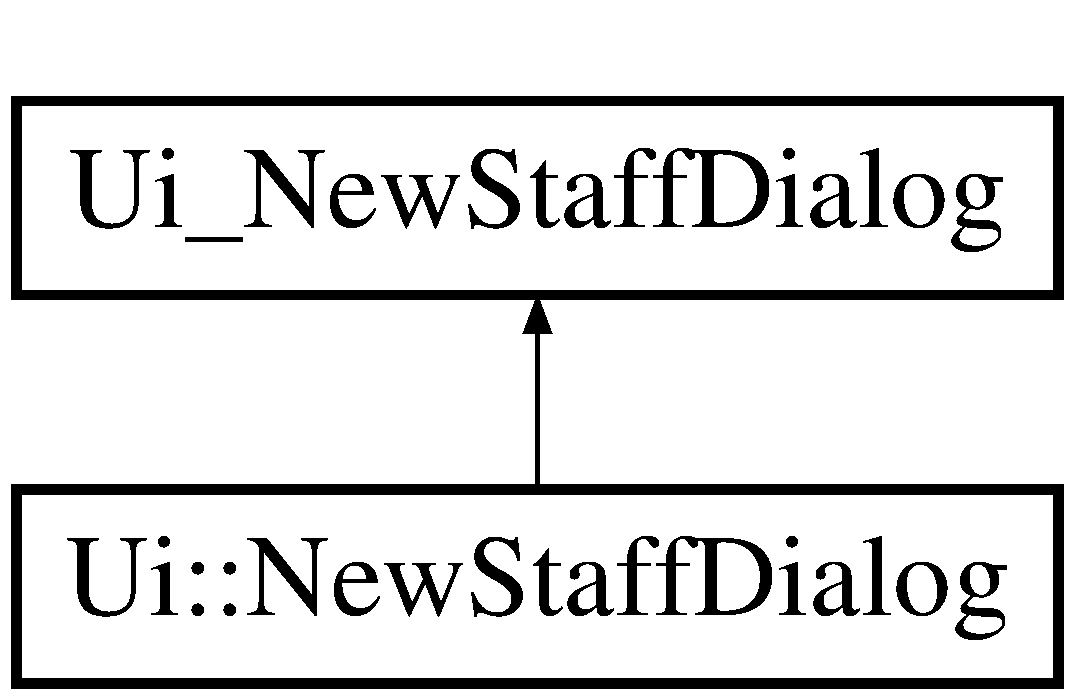
\includegraphics[height=2.000000cm]{class_ui___new_staff_dialog}
\end{center}
\end{figure}
\subsection*{Public Member Functions}
\begin{DoxyCompactItemize}
\item 
\hypertarget{class_ui___new_staff_dialog_afd350b5820fa472c7d4e7b2bf57d8620}{}void {\bfseries setup\+Ui} (Q\+Dialog $\ast$\hyperlink{class_new_staff_dialog}{New\+Staff\+Dialog})\label{class_ui___new_staff_dialog_afd350b5820fa472c7d4e7b2bf57d8620}

\item 
\hypertarget{class_ui___new_staff_dialog_aa5cebfdc19be78310c286e5e77e99133}{}void {\bfseries retranslate\+Ui} (Q\+Dialog $\ast$\hyperlink{class_new_staff_dialog}{New\+Staff\+Dialog})\label{class_ui___new_staff_dialog_aa5cebfdc19be78310c286e5e77e99133}

\end{DoxyCompactItemize}
\subsection*{Public Attributes}
\begin{DoxyCompactItemize}
\item 
\hypertarget{class_ui___new_staff_dialog_a1bade48a910d0af18f039b4a78a948d3}{}Q\+Dialog\+Button\+Box $\ast$ {\bfseries button\+Box}\label{class_ui___new_staff_dialog_a1bade48a910d0af18f039b4a78a948d3}

\item 
\hypertarget{class_ui___new_staff_dialog_a42b05728e0042c530fd8543bb2a9c2f5}{}Q\+Group\+Box $\ast$ {\bfseries group\+Box}\label{class_ui___new_staff_dialog_a42b05728e0042c530fd8543bb2a9c2f5}

\item 
\hypertarget{class_ui___new_staff_dialog_aadd7fb749e7a9110930d383f5efc1b59}{}Q\+Widget $\ast$ {\bfseries layout\+Widget}\label{class_ui___new_staff_dialog_aadd7fb749e7a9110930d383f5efc1b59}

\item 
\hypertarget{class_ui___new_staff_dialog_a170f1fc421a1fe9b257284b4e9fe9868}{}Q\+V\+Box\+Layout $\ast$ {\bfseries vertical\+Layout}\label{class_ui___new_staff_dialog_a170f1fc421a1fe9b257284b4e9fe9868}

\item 
\hypertarget{class_ui___new_staff_dialog_ad943fea135f1de374ab7e0d5a7cceb99}{}Q\+Radio\+Button $\ast$ {\bfseries treble\+Radio\+Button}\label{class_ui___new_staff_dialog_ad943fea135f1de374ab7e0d5a7cceb99}

\item 
\hypertarget{class_ui___new_staff_dialog_a5792d1039e7a6c325cdc56afdafd3a5d}{}Q\+Radio\+Button $\ast$ {\bfseries alto\+Radio\+Button}\label{class_ui___new_staff_dialog_a5792d1039e7a6c325cdc56afdafd3a5d}

\item 
\hypertarget{class_ui___new_staff_dialog_a5d0bc85905731c6e38163152edf6288c}{}Q\+Radio\+Button $\ast$ {\bfseries tenor\+Radio\+Button}\label{class_ui___new_staff_dialog_a5d0bc85905731c6e38163152edf6288c}

\item 
\hypertarget{class_ui___new_staff_dialog_ab4325885d3c5b5793266c05af4899a05}{}Q\+Radio\+Button $\ast$ {\bfseries bass\+Radio\+Button}\label{class_ui___new_staff_dialog_ab4325885d3c5b5793266c05af4899a05}

\item 
\hypertarget{class_ui___new_staff_dialog_a5f1120f8e1c3fc71443eb6a7bec24df5}{}Q\+Group\+Box $\ast$ {\bfseries group\+Box\+\_\+2}\label{class_ui___new_staff_dialog_a5f1120f8e1c3fc71443eb6a7bec24df5}

\item 
\hypertarget{class_ui___new_staff_dialog_a556d00ef21ad74c2de3c2d52c929e2dc}{}Q\+Combo\+Box $\ast$ {\bfseries combo\+Box}\label{class_ui___new_staff_dialog_a556d00ef21ad74c2de3c2d52c929e2dc}

\end{DoxyCompactItemize}


The documentation for this class was generated from the following file\+:\begin{DoxyCompactItemize}
\item 
C\+:/\+Users/kollg/\+Documents/\+Git\+Hub/\+Counterpoint-\/project/ui\+\_\+newstaffdialog.\+h\end{DoxyCompactItemize}

\hypertarget{class_v_note}{}\section{V\+Note Class Reference}
\label{class_v_note}\index{V\+Note@{V\+Note}}
Inheritance diagram for V\+Note\+:\begin{figure}[H]
\begin{center}
\leavevmode
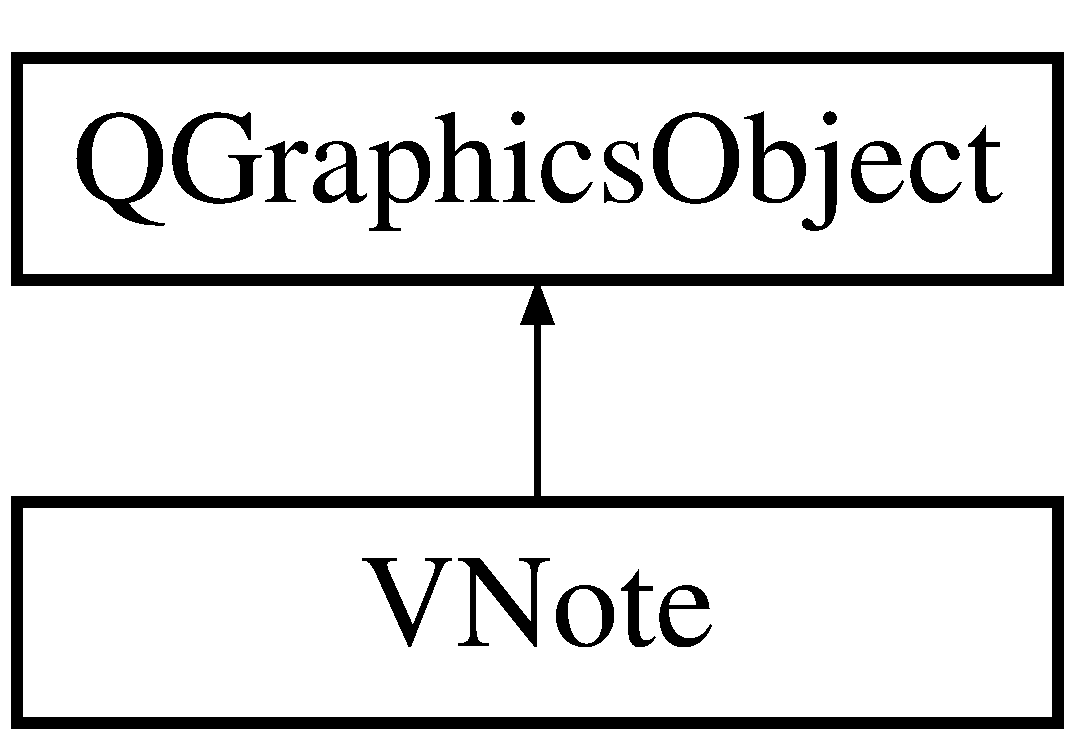
\includegraphics[height=2.000000cm]{class_v_note}
\end{center}
\end{figure}
\subsection*{Public Slots}
\begin{DoxyCompactItemize}
\item 
\hypertarget{class_v_note_af25595b327a49fd2ee53332634f5480d}{}void {\bfseries hover\+Entered} (\hyperlink{class_v_staff_line}{V\+Staff\+Line} $\ast$staffline)\label{class_v_note_af25595b327a49fd2ee53332634f5480d}

\end{DoxyCompactItemize}
\subsection*{Signals}
\begin{DoxyCompactItemize}
\item 
\hypertarget{class_v_note_a3f78010b5f01c260cd8b317fb6e57ec1}{}void {\bfseries v\+Note\+Selecting} (\hyperlink{class_v_note}{V\+Note} $\ast$note)\label{class_v_note_a3f78010b5f01c260cd8b317fb6e57ec1}

\item 
\hypertarget{class_v_note_a9ecb1c67b0c0c61afd07c11f642819e6}{}void {\bfseries v\+Note\+Pos\+Changing} (\hyperlink{class_v_note}{V\+Note} $\ast$note)\label{class_v_note_a9ecb1c67b0c0c61afd07c11f642819e6}

\end{DoxyCompactItemize}
\subsection*{Public Member Functions}
\begin{DoxyCompactItemize}
\item 
\hypertarget{class_v_note_ae8c4cf09c4846142f0fb29277c3ec27a}{}{\bfseries V\+Note} (bool newnote=false, unsigned int spos=0, Score\+View\+Model\+::note\+Types ntype=Score\+View\+Model\+::half, Score\+View\+Model\+::accents acc=Score\+View\+Model\+::none, Q\+Graphics\+Object $\ast$parent=0)\label{class_v_note_ae8c4cf09c4846142f0fb29277c3ec27a}

\item 
\hypertarget{class_v_note_a0c2d23d2544e6c898d022c43a9a415bb}{}Q\+Rect\+F {\bfseries bounding\+Rect} () const \label{class_v_note_a0c2d23d2544e6c898d022c43a9a415bb}

\item 
\hypertarget{class_v_note_ad128b6e755d08912b725445f66759860}{}void {\bfseries paint} (Q\+Painter $\ast$painter, const Q\+Style\+Option\+Graphics\+Item $\ast$option, Q\+Widget $\ast$widget)\label{class_v_note_ad128b6e755d08912b725445f66759860}

\item 
\hypertarget{class_v_note_aa867aa12bc455041eb5e84b3cf9828f5}{}int {\bfseries get\+Scorepos} () const \label{class_v_note_aa867aa12bc455041eb5e84b3cf9828f5}

\item 
\hypertarget{class_v_note_a9c476ddccb3cb3e3573688bd4956c89b}{}void {\bfseries set\+Scorepos} (int value)\label{class_v_note_a9c476ddccb3cb3e3573688bd4956c89b}

\item 
\hypertarget{class_v_note_a31d3c808548e1f768c25b1a2f84c536d}{}void {\bfseries change\+To\+Rest} ()\label{class_v_note_a31d3c808548e1f768c25b1a2f84c536d}

\item 
\hypertarget{class_v_note_a36b8c39a29fffc4de5fdb4a1073871b8}{}Score\+View\+Model\+::note\+Types {\bfseries get\+Notetype} () const \label{class_v_note_a36b8c39a29fffc4de5fdb4a1073871b8}

\item 
\hypertarget{class_v_note_ac043ebad591f4d5b5506f3ab7d0b6b63}{}void {\bfseries set\+Notetype} (const Score\+View\+Model\+::note\+Types \&value)\label{class_v_note_ac043ebad591f4d5b5506f3ab7d0b6b63}

\item 
\hypertarget{class_v_note_a322432eef57f6c69b10695305c123100}{}Score\+View\+Model\+::accents {\bfseries get\+Accent} () const \label{class_v_note_a322432eef57f6c69b10695305c123100}

\item 
\hypertarget{class_v_note_ad2efcba0091075d64e19bd01fa69817d}{}void {\bfseries set\+Accent} (const Score\+View\+Model\+::accents \&value)\label{class_v_note_ad2efcba0091075d64e19bd01fa69817d}

\end{DoxyCompactItemize}
\subsection*{Protected Member Functions}
\begin{DoxyCompactItemize}
\item 
\hypertarget{class_v_note_ae584af522ce182ec7919b0802e2aaf6b}{}void {\bfseries mouse\+Press\+Event} (Q\+Graphics\+Scene\+Mouse\+Event $\ast$event)\label{class_v_note_ae584af522ce182ec7919b0802e2aaf6b}

\item 
\hypertarget{class_v_note_aef4d0e27761e5a423fca0befd1e118e0}{}void {\bfseries mouse\+Move\+Event} (Q\+Graphics\+Scene\+Mouse\+Event $\ast$event)\label{class_v_note_aef4d0e27761e5a423fca0befd1e118e0}

\item 
\hypertarget{class_v_note_a2335dbb188102ea316bbc79609f8e2fb}{}void {\bfseries mouse\+Release\+Event} (Q\+Graphics\+Scene\+Mouse\+Event $\ast$event)\label{class_v_note_a2335dbb188102ea316bbc79609f8e2fb}

\end{DoxyCompactItemize}


The documentation for this class was generated from the following files\+:\begin{DoxyCompactItemize}
\item 
C\+:/\+Users/kollg/\+Documents/\+Git\+Hub/\+Counterpoint-\/project/vnote.\+h\item 
C\+:/\+Users/kollg/\+Documents/\+Git\+Hub/\+Counterpoint-\/project/vnote.\+cpp\end{DoxyCompactItemize}

\hypertarget{class_v_staff}{}\section{V\+Staff Class Reference}
\label{class_v_staff}\index{V\+Staff@{V\+Staff}}
Inheritance diagram for V\+Staff\+:\begin{figure}[H]
\begin{center}
\leavevmode
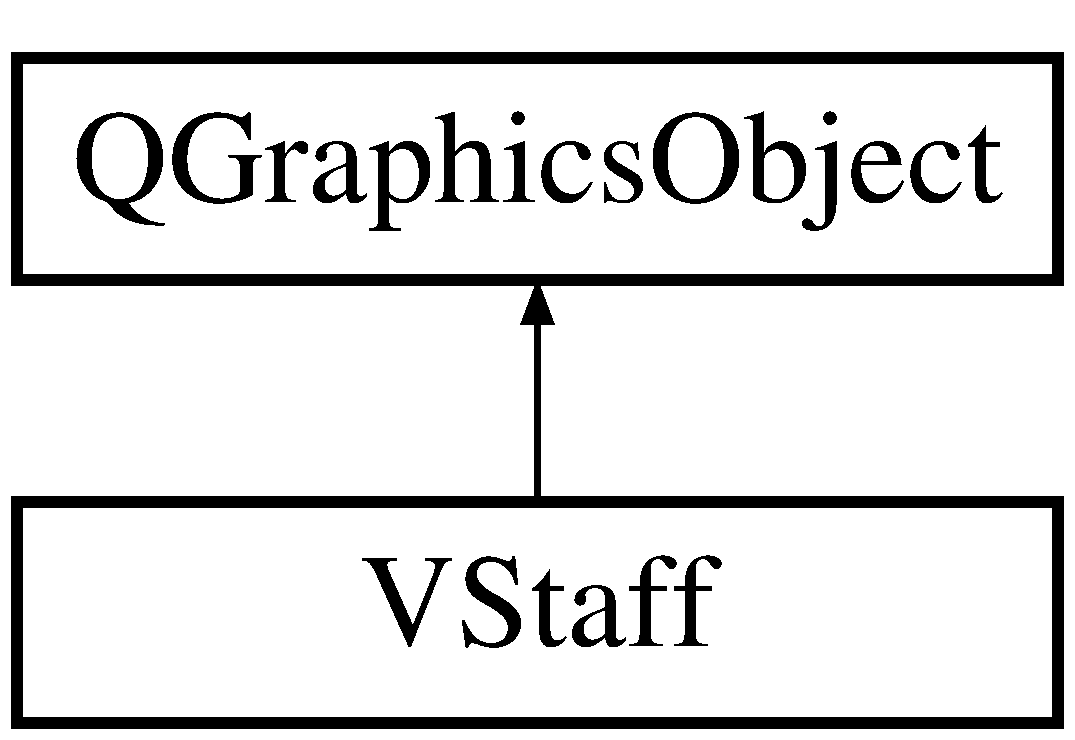
\includegraphics[height=2.000000cm]{class_v_staff}
\end{center}
\end{figure}
\subsection*{Signals}
\begin{DoxyCompactItemize}
\item 
\hypertarget{class_v_staff_a79cbbcba090397f001af49c89516d88e}{}void {\bfseries vstaff\+Select} (\hyperlink{class_v_staff}{V\+Staff} $\ast$vstaff)\label{class_v_staff_a79cbbcba090397f001af49c89516d88e}

\item 
\hypertarget{class_v_staff_a7cb560594badc35f609ed4dc183ab030}{}void {\bfseries new\+V\+Note\+Add} (\hyperlink{class_v_note}{V\+Note} $\ast$vnote)\label{class_v_staff_a7cb560594badc35f609ed4dc183ab030}

\end{DoxyCompactItemize}
\subsection*{Public Member Functions}
\begin{DoxyCompactItemize}
\item 
\hypertarget{class_v_staff_af020580c558ab24a9af2bccbab36ec33}{}{\bfseries V\+Staff} (Score\+View\+Model\+::clef\+Names clef=Score\+View\+Model\+::treble, \hyperlink{class_key_signature}{Key\+Signature} keysig=0, Q\+Graphics\+Object $\ast$parent=0)\label{class_v_staff_af020580c558ab24a9af2bccbab36ec33}

\item 
\hypertarget{class_v_staff_ade19faa451d9ce058cddcafeacb5a432}{}Q\+Rect\+F {\bfseries bounding\+Rect} () const \label{class_v_staff_ade19faa451d9ce058cddcafeacb5a432}

\item 
\hypertarget{class_v_staff_aeefc796be13d05ddc8bfee7ff49ee5b6}{}void {\bfseries paint} (Q\+Painter $\ast$painter, const Q\+Style\+Option\+Graphics\+Item $\ast$option, Q\+Widget $\ast$widget)\label{class_v_staff_aeefc796be13d05ddc8bfee7ff49ee5b6}

\item 
\hypertarget{class_v_staff_af6260222d1f6c5af860edeee4e5ad2e2}{}Q\+List$<$ \hyperlink{class_v_staff_line}{V\+Staff\+Line} $\ast$ $>$ {\bfseries get\+Vstafflines} () const \label{class_v_staff_af6260222d1f6c5af860edeee4e5ad2e2}

\item 
\hypertarget{class_v_staff_a37e2606c7ff7e487059337274c706c2b}{}Q\+List$<$ \hyperlink{class_v_note}{V\+Note} $\ast$ $>$ {\bfseries get\+Vnotes} () const \label{class_v_staff_a37e2606c7ff7e487059337274c706c2b}

\item 
\hypertarget{class_v_staff_af0e303b975eb997e6e11bd7696bf8ead}{}void {\bfseries show\+Next\+V\+Note} (\hyperlink{class_v_note}{V\+Note} $\ast$vnote)\label{class_v_staff_af0e303b975eb997e6e11bd7696bf8ead}

\item 
\hypertarget{class_v_staff_a7ca9cc1d027b2796047aff5020fa195b}{}void {\bfseries set\+New\+V\+Note} (Score\+View\+Model\+::note\+Types notetype, Score\+View\+Model\+::accents accent)\label{class_v_staff_a7ca9cc1d027b2796047aff5020fa195b}

\item 
\hypertarget{class_v_staff_a5560aebaca63c903d6514674a090716a}{}void {\bfseries add\+New\+V\+Note} ()\label{class_v_staff_a5560aebaca63c903d6514674a090716a}

\item 
\hypertarget{class_v_staff_ac7e53a5a6092b7b57ab0a1f36d2357d9}{}void {\bfseries delete\+Selected\+V\+Note} ()\label{class_v_staff_ac7e53a5a6092b7b57ab0a1f36d2357d9}

\item 
\hypertarget{class_v_staff_ad42533b9604fd8abec281dcf6d1be8ee}{}\hyperlink{class_v_note}{V\+Note} $\ast$ {\bfseries get\+Newvnote} () const \label{class_v_staff_ad42533b9604fd8abec281dcf6d1be8ee}

\item 
\hypertarget{class_v_staff_a2b8d021fd00eaf7e4fda38a2c58b8d9e}{}void {\bfseries set\+Newvnote} (\hyperlink{class_v_note}{V\+Note} $\ast$value)\label{class_v_staff_a2b8d021fd00eaf7e4fda38a2c58b8d9e}

\item 
\hypertarget{class_v_staff_aaf1790a96768e184d2b6c1299d4eb230}{}Score\+View\+Model\+::clef\+Names {\bfseries get\+Clef} () const \label{class_v_staff_aaf1790a96768e184d2b6c1299d4eb230}

\item 
\hypertarget{class_v_staff_ae38cc7590d13e6992e996c91dd209cb4}{}\hyperlink{class_v_note}{V\+Note} $\ast$ {\bfseries get\+Selectedvnote} () const \label{class_v_staff_ae38cc7590d13e6992e996c91dd209cb4}

\item 
\hypertarget{class_v_staff_a2c1531ee4734bccf5ffe7bd66f988583}{}void {\bfseries set\+Selectedvnote} (\hyperlink{class_v_note}{V\+Note} $\ast$value)\label{class_v_staff_a2c1531ee4734bccf5ffe7bd66f988583}

\item 
\hypertarget{class_v_staff_ac96715515c3f55229ba114293ece82fd}{}void {\bfseries update\+Staff\+Width} ()\label{class_v_staff_ac96715515c3f55229ba114293ece82fd}

\item 
\hypertarget{class_v_staff_aa4d00861f977630d44c8c19a09c05da5}{}void {\bfseries update\+V\+Staff} ()\label{class_v_staff_aa4d00861f977630d44c8c19a09c05da5}

\item 
\hypertarget{class_v_staff_a95b415e2f53afe972263f62149203710}{}\hyperlink{class_key_signature}{Key\+Signature} {\bfseries get\+Keysignature} () const \label{class_v_staff_a95b415e2f53afe972263f62149203710}

\end{DoxyCompactItemize}
\subsection*{Protected Member Functions}
\begin{DoxyCompactItemize}
\item 
\hypertarget{class_v_staff_a570bacf43a4ba401525bda3b037d3c0d}{}void {\bfseries mouse\+Press\+Event} (Q\+Graphics\+Scene\+Mouse\+Event $\ast$event)\label{class_v_staff_a570bacf43a4ba401525bda3b037d3c0d}

\end{DoxyCompactItemize}


The documentation for this class was generated from the following files\+:\begin{DoxyCompactItemize}
\item 
C\+:/\+Users/kollg/\+Documents/\+Git\+Hub/\+Counterpoint-\/project/vstaff.\+h\item 
C\+:/\+Users/kollg/\+Documents/\+Git\+Hub/\+Counterpoint-\/project/vstaff.\+cpp\end{DoxyCompactItemize}

\hypertarget{class_v_staff_line}{}\section{V\+Staff\+Line Class Reference}
\label{class_v_staff_line}\index{V\+Staff\+Line@{V\+Staff\+Line}}
Inheritance diagram for V\+Staff\+Line\+:\begin{figure}[H]
\begin{center}
\leavevmode
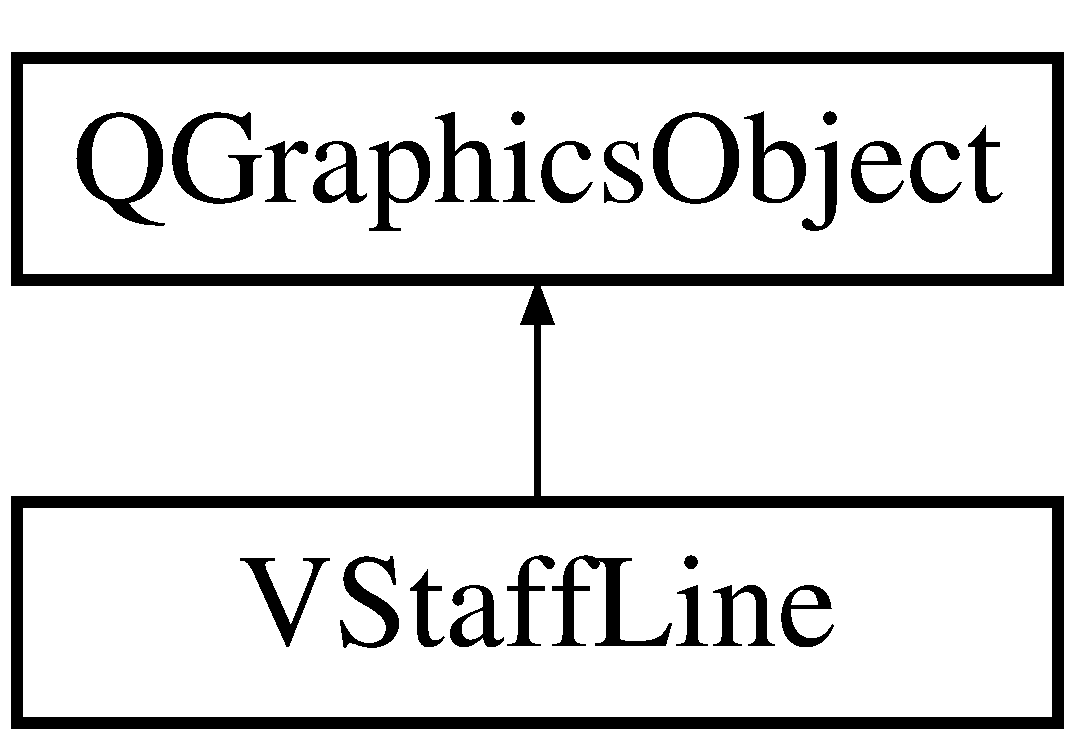
\includegraphics[height=2.000000cm]{class_v_staff_line}
\end{center}
\end{figure}
\subsection*{Signals}
\begin{DoxyCompactItemize}
\item 
\hypertarget{class_v_staff_line_ab68a189c08552b4c039f904ecd339e71}{}void {\bfseries hover\+Entering} (\hyperlink{class_v_staff_line}{V\+Staff\+Line} $\ast$staffline)\label{class_v_staff_line_ab68a189c08552b4c039f904ecd339e71}

\end{DoxyCompactItemize}
\subsection*{Public Member Functions}
\begin{DoxyCompactItemize}
\item 
\hypertarget{class_v_staff_line_aec47a7b0b853e3e8ec8d0cc527088db1}{}{\bfseries V\+Staff\+Line} (bool iswhite=true, int initstaffwidth=173, Q\+Graphics\+Object $\ast$parent=0)\label{class_v_staff_line_aec47a7b0b853e3e8ec8d0cc527088db1}

\item 
\hypertarget{class_v_staff_line_ae2e42820d76de2c34f1f546fd1dde643}{}Q\+Rect\+F {\bfseries bounding\+Rect} () const \label{class_v_staff_line_ae2e42820d76de2c34f1f546fd1dde643}

\item 
\hypertarget{class_v_staff_line_a9bf019b9c17fc3d64634127eed4682c8}{}void {\bfseries paint} (Q\+Painter $\ast$painter, const Q\+Style\+Option\+Graphics\+Item $\ast$option, Q\+Widget $\ast$widget)\label{class_v_staff_line_a9bf019b9c17fc3d64634127eed4682c8}

\item 
\hypertarget{class_v_staff_line_ae64934fb567dedfef9cd9acdc8bce4b0}{}void {\bfseries add\+Staffwidth} (int value)\label{class_v_staff_line_ae64934fb567dedfef9cd9acdc8bce4b0}

\end{DoxyCompactItemize}
\subsection*{Protected Member Functions}
\begin{DoxyCompactItemize}
\item 
\hypertarget{class_v_staff_line_aa1c1f06139ef4647c7555c1c2693eb15}{}void {\bfseries hover\+Enter\+Event} (Q\+Graphics\+Scene\+Hover\+Event $\ast$event)\label{class_v_staff_line_aa1c1f06139ef4647c7555c1c2693eb15}

\end{DoxyCompactItemize}


The documentation for this class was generated from the following files\+:\begin{DoxyCompactItemize}
\item 
C\+:/\+Users/kollg/\+Documents/\+Git\+Hub/\+Counterpoint-\/project/vstaffline.\+h\item 
C\+:/\+Users/kollg/\+Documents/\+Git\+Hub/\+Counterpoint-\/project/vstaffline.\+cpp\end{DoxyCompactItemize}

%--- End generated contents ---

% Index
\backmatter
\newpage
\phantomsection
\clearemptydoublepage
\addcontentsline{toc}{chapter}{Index}
\printindex

\end{document}
